\section{Программная реализация метода безопасности водителя}
\subsection{Средства реализации программного комплекса}
\subsubsection{Выбор языка программирования}
Для написания программного комплекса  был выбран язык программирования Python \cite{python}, так как он обладает следующими критериями:
\begin{itemize}[leftmargin=1.6\parindent]
	\item[--] большое количество библиотек для работы с нейронными сетями;
	\item[--] возможность создавать графические интерфейсы;
	\item[--] возможность тренировать модель нейронной сети на графическом процессоре.
\end{itemize}

\subsubsection{Выбор библиотеки для работы с нейронной сетью}
Для реализации и обучения модели нейронной сети была выбрана библиотека tensorflow \cite{tensorflow}, так как является наиболее часто используемой и требует меньшего времени для обучения модели по сравнению с второй по популярности библиотекой PyTorch \cite{tensorflow_pytorch}.

\subsection{Реализация программного комплекса}
Модули метода оценки и загрузки данных представлены в листингах \ref{lst:main} и \ref{lst:get_img} соответственно. Далее будут подробно рассмотрены модули пользовательского интерфейса и GoogleNet модели.

\subsubsection{Модуль пользовательского интерфейса}
Интерфейс пользовательского приложения при запуске представлен на рисунке \ref{fig:example_app}.
\begin{figure}[hbtp]
	\centering
	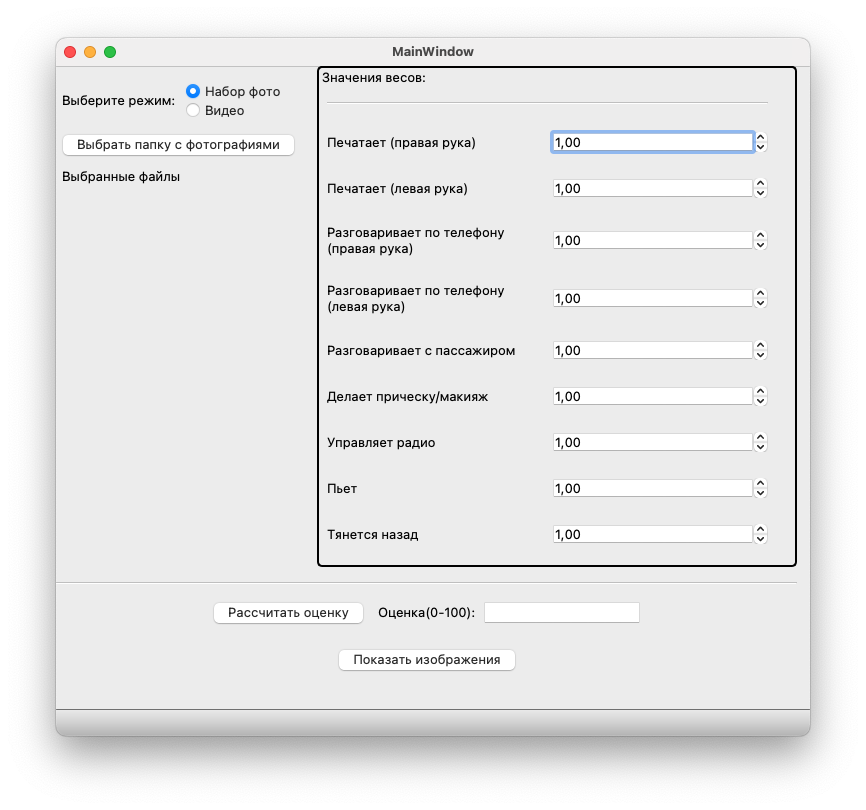
\includegraphics[scale=0.55]{img/example_app.png}
	\caption{Пользовательское приложение}
	\label{fig:example_app}
\end{figure}
\clearpage

\subsubsection{Модуль GoogleNet модели}
Реализация модели построена на классической GoogleNet модели с 9 $incep-tion$ блоками и 2 вспомогательными классификаторами. Вспомогательные классификаторы обеспечивают более эффективную и стабильную сходимость обучения.

В листинге \ref{lst:googlenet} приведена реализация модели GoogleNet, отвечающая за классификацию изображений.

У модели 3 выхода, 1 основной и 2 вспомогательных (засчет дополнительных классификаторов). Результат работы модели берется из основного выхода. Каждый выход представляет собой массив из 10 (количество классов) чисел (вероятностей). В данной работе класс с наибольшей вероятностью считается достоверным.

\subsubsection{Обучение модели}
Перед обучением модели необходимо произвести конвертацию исходных изображений к размеру 224 × 224 пикселей и формату RGB как этого требует модель.

В процессе обучения тренировочные данные подвергаются преобразованиям, таким как отражение, переворот, масштабирование. Это позволяет расширить набор тренировочных данных и повысить точность модели.

Обучение производилось на облачном NVIDIA DGX \cite{dgx} сервере, с графическим процессором NVIDIA Tesla V100 имеющий 32 гигабайта видеопамяти.

В листинге \ref{lst:train} приведена реализация процесса обучения реализованной модели GoogleNet.
Пример классификации представлен на рисунках \ref{fig:train_example_1} --- \ref{fig:train_example_2}

\begin{figure}[hbtp]
	\centering
	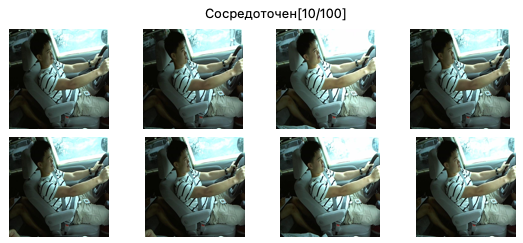
\includegraphics[scale=0.8]{img/train_example.png}
	\caption{Пример классификации, класс <<Сосредоточен>>}
	\label{fig:train_example_1}
\end{figure}

\begin{figure}[hbtp]
	\centering
	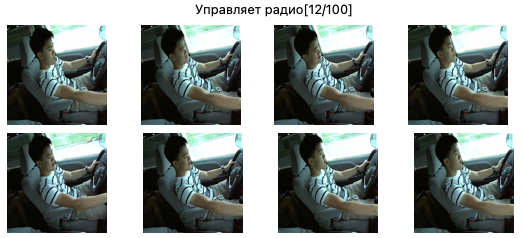
\includegraphics[scale=0.8]{img/train_example_2.png}
	\caption{Пример классификации, класс <<Управляет радио>>}
	\label{fig:train_example_2}
\end{figure}

Обучение производилось в течение 200 итераций (эпох), каждая эпоха состояла из 180 шагов. Набор данных для обучения был разделен на обучающий и валидационный в соотношении 4 к 1 соответственно. Валидационная часть набора нужна для того, чтобы можно оценить точность модели в конце каждой эпохи на данных, неучавствующих в обучении.

\subsubsection{Результаты обучения модели}
На рисунках \ref{fig:train_acc} и \ref{fig:val_acc} представлены метрики точности на обучающих и валидационнах данных соответственно. Стоит отметить, что точность модели начала расти только после 30 эпох на обоих наборах данных и достигла 100 процентов на обучающих данных и 98 процентов на валидационных.

\begin{figure}[hbtp]
	\centering
	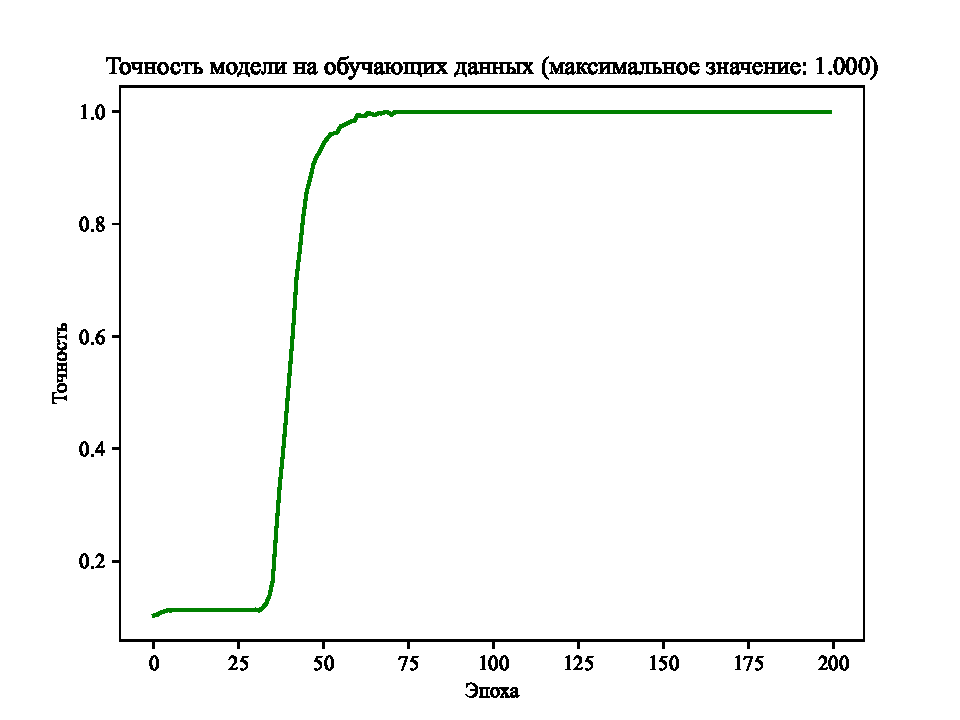
\includegraphics[scale=0.8]{img/train_accuracy.pdf}
	\caption{Точность модели на обучающих данных}
	\label{fig:train_acc}
\end{figure}

\begin{figure}[hbtp]
	\centering
	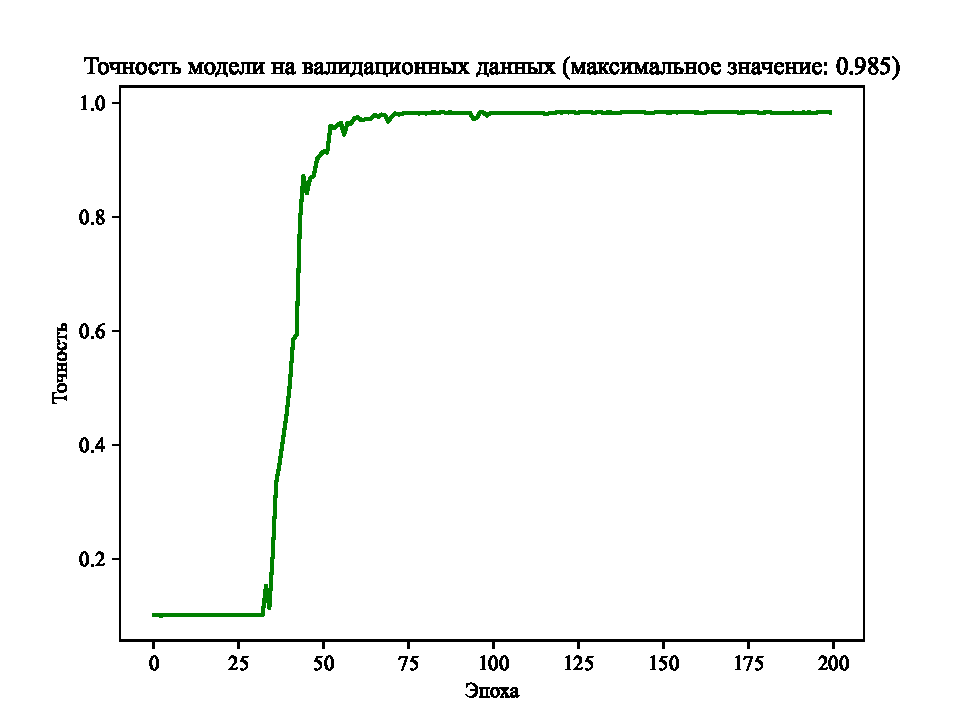
\includegraphics[scale=0.8]{img/val_accuracy.pdf}
	\caption{Точность модели на валидационных данных}
	\label{fig:val_acc}
\end{figure}
\clearpage


\subsection{Примеры использования разработанного программного комплекса}
Модуль модели GoogleNet представляет собой скрипт на языке программирования python, выполняющий обучение модели. Запуск данного скрипта осуществляется через консоль. Пример запуска модуля для обучения модели представлен в листинге \ref{lst:train_start}. Различные параметры, такие как количество эпох, путь до папки с набором данных можно изменить непосредственно в программном коде, они представлены как константы.

\lstinputlisting[
caption={Запуск обучения модели},
label={lst:train_start},
language=python
]{code/train_start.txt}

Модуль пользовательского интерфейса представляет собой графический интерфейс, запуск которого также производится через терминал. 

После выбора режима нужно выбрать либо папку с фотографиями либо видеофайл на диске, затем в приложении в интерфейсе приложения будет продублирован выбранный путь как на рисунке \ref{fig:example_app_1}.

\begin{figure}[hbtp]
	\centering
	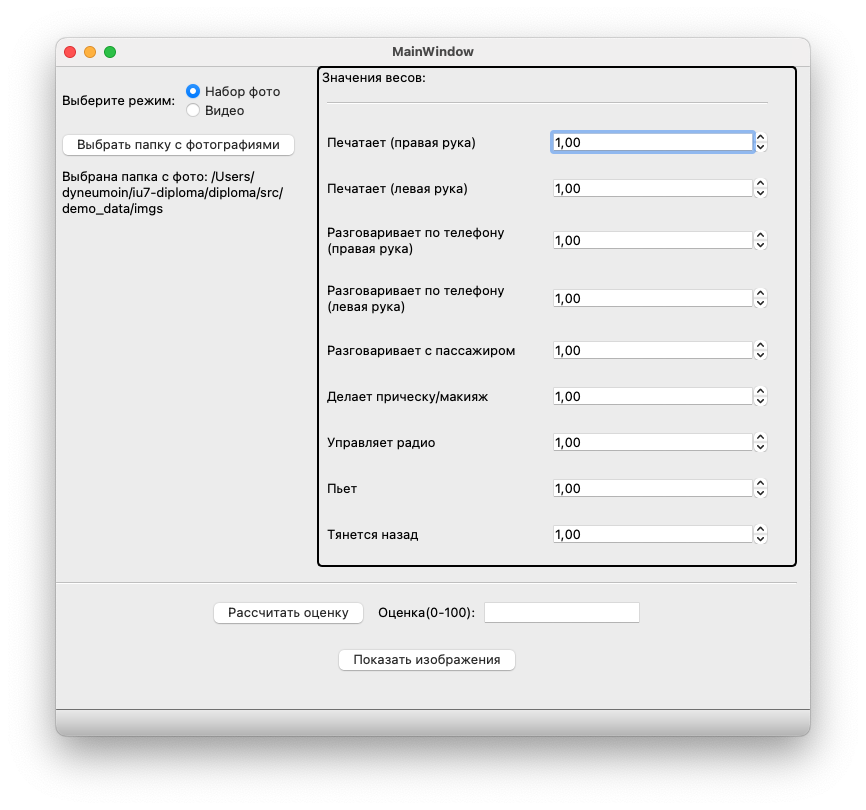
\includegraphics[scale=0.55]{img/example_app_1.png}
	\caption{Пользовательское приложение (выбран путь к изображениям)}
	\label{fig:example_app_1}
\end{figure}
\clearpage

После выбора пути к изображениям или видеофайлу можно рассчитать оценку, нажав на соответствующую кнопку <<Рассчитать оценку>>, значение оценки отобразится в поле с заголовком <<Оценка(0-100)>> как на рисунке \ref{fig:example_app_2}.

\begin{figure}[hbtp]
	\centering
	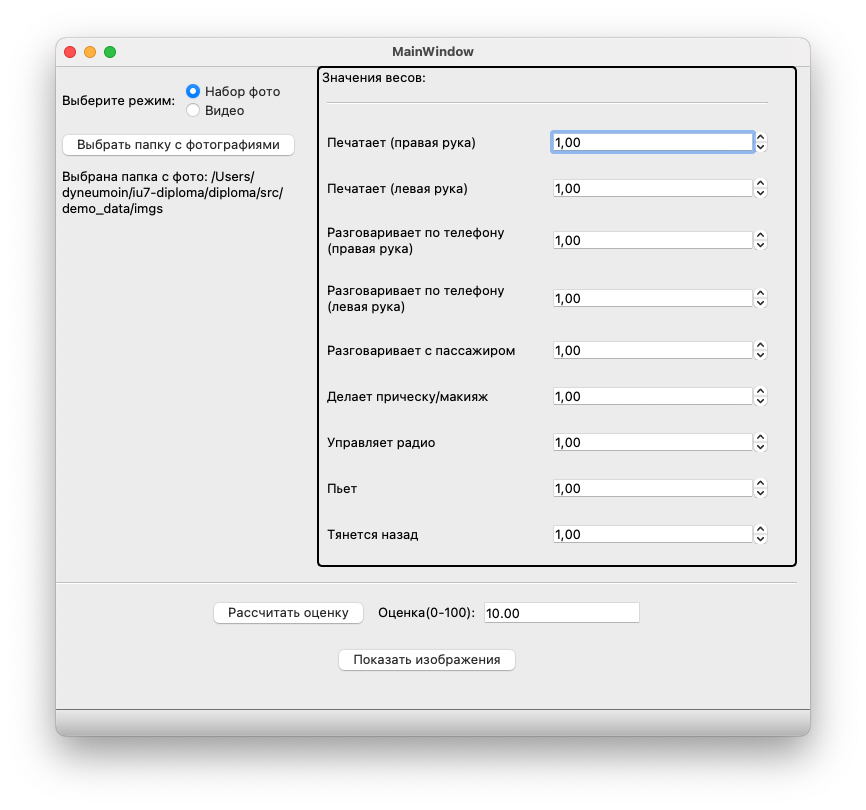
\includegraphics[scale=0.55]{img/example_app_2.png}
	\caption{Пользовательское приложение (рассчитана оценка)}
	\label{fig:example_app_2}
\end{figure}
\clearpage

Если требуется просмотреть изображения, разделенные по классам, то это можно сделать по нажатию кнопки <<Показать изображения>>, откроется отдельное диалоговое окно с группами классов, в начале группы будет название класса и количество в формате [количество изображений класса / общее количество изображений] как на рисунке \ref{fig:example_app_3}.

\begin{figure}[hbtp]
	\centering
	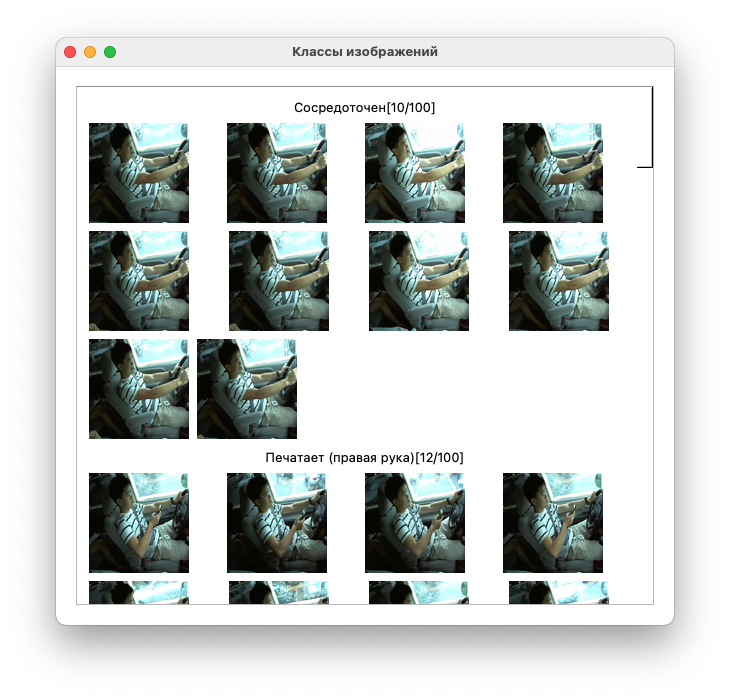
\includegraphics[scale=0.55]{img/example_app_3.png}
	\caption{Пользовательское приложение (диалоговое окно с изображениями)}
	\label{fig:example_app_3}
\end{figure}
\clearpage

\subsection*{Вывод}
Были описаны средства реализации программного комплекса. Приведены листинги реализации каждого компонента комплекса, примеры работы компонентов, их входные и выходные данные. Описаны технологии и методы, использовавшиеся при реализации. Представлены примеры взаимодействия с модулями.

\pagebreak